\setcounter{chapter}{0}
\chapter{绪论}
\section{物质形态与空气动力学定义}
\thispagestyle{empty}	
\subsection{物质形态}
\noindent  自然界主要存在3种形态:
\begin{enumerate}
	\item \dy[固体]{GT}:具有固定的体积,无固定的形状。在静止状态下,可以承受垂直于表面的压力、水平拉力和剪切力。\vspace*{-0.5em}
	\item \dy[液体]{YT}:具有固定的体积,无固定的形状。在静止状态下,只能承受垂直于表面的压力,几乎没有水平拉力和剪切力。\vspace*{-0.5em}
	\item \dy[气体]{QT}:没有固定的体积,也没有固定的形状。在静止状态下,只能承受垂直于表面的压力,几乎没有水平拉力和剪切力。\vspace*{-0.5em}
\end{enumerate}

\subsection{空气动力学的定义}
\begin{equation*}
	\mbox{流体力学} \, 
	\begin{cases}
		\, \mbox{流体动力学}\,
		\begin{cases}
			\, \mbox{水动力学} \\
			\, \mbox{\textcolor{red}{空气动力学}}
		\end{cases}\\
		\, \mbox{流体静力学}
	\end{cases}
\end{equation*}

空气动力学是流体力学的一个分支,他是从流体力学发展而来。

\dy[流体力学]{LTLX}是研究流体(水、空气、石油等)平衡和机械运动的规律及其应用的学科。

\defination[空气动力学]
{\dy[空气动力学]{KQDLX}是研究物体和空气作\textcolor{blue}{相对运动}时,空气的运动规律以及空气与物体之间的相对运动关系的学科。}

\subsection{空气动力学的分类}
\begin{equation*}
	\mbox{空气动力学}\, 
	\begin{cases}
		\mbox{高速空气动力学(可压流或气体动力学)} \,
		\begin{cases}
			\, \mbox{亚声速空气动力学}\\
			\, \mbox{跨声速空气动力学}\\
			\, \mbox{超声速空气动力学}
		\end{cases}\\
	\mbox{低速空气动力学(不可压流,类似于水)}
	\end{cases}
\end{equation*}

\section{相对飞行理论}

\section{空气动力学的研究方法}
\subsection{理论分析}
\begin{enumerate}
	\item 建立合理的理论模型
\end{enumerate}
\subsection{数值模拟}
\begin{itemize}
	\item 理论控制方程的近似求解方法—空间和时间的离散
	\item 常用的求解方法:有限元
\end{itemize}
\subsection{实验研究}
主要依靠风洞实验设施。




\chapter{流体物理属性与静力学}
\section{流体的属性}
\thispagestyle{empty}
\subsection{连续介质假设}
\begin{itemize}
	\item 从微观上看
	\begin{itemize}
		\item 流体分子的运动具有不均匀、离散和随机特性
		\item 不论是液体还是气体,分子之间都存在间隙。但是由于分子的\dy[平均自由程$I$]{PJZYC}与研究的对象的尺寸$L$相比可以忽略不计。
	\end{itemize}
	\item 从宏观上看
	\begin{itemize}
		\item 分布均匀且运动连续和确定(速度、压强、密度和温度分布场)。
	\end{itemize}
\end{itemize}

\defination[连续介质]
{
	当受到扰动时介质(流体)所表现出的是大量分子运动体现出的宏观特性(如速度 、 压强 、 密度 、 温度等)的\red[均匀性] 、\red[连续性]和\red[确定性]变化,这种介质定义为\dy[连续介质]{LXJZ}。
}

\dyb[流体质点]\index{LTZD@流体质点} 一个微观上充分大(分子尺度),宏观上充分小(物体尺度)的分子团(无穷多个分子),是\blue{宏观上组成流体的最小单元},流体质点所具有的宏观物理量\blue{满足一切物理定律}。
\vspace*{0.5em}

\theorem[流体的连续介质假设]
{流体是由\textcolor{red}{连续无间隙}地\textcolor{red}{均匀充满}所占空间的\textcolor{blue}{流体质点}组成。}

根据连续性假设的条件下,流体介质某点的密度可以表示为
\begin{equation}
	\rho = \lim\limits_{\Delta \nu \to \Delta \nu_0}\dfrac{\Delta m}{\Delta \nu}
\end{equation}

而在数学上,应该是$\Delta \tau \to 0$,但由于在物理微观条件下,当$\Delta \tau$足够小的时候,就体现分子性,从而使得密度不连续,而是离散的,如图\ref{连续密度}所示。但是,从宏观的角度来看,$\Delta \nu_0 $可以看作0,即
\begin{equation}
	\rho = \lim\limits_{\Delta \nu \to 0}\dfrac{\Delta m}{\Delta \nu}
\end{equation}
\vspace*{-2em}

\warn
[	
\hspace*{2em} 在连续介质观点的假设下,流体的最小体积单元为质点(不是分子,也不是分子微团)。连续性假设的成立条件是:分子的尺寸远大于分子自由程(一般要求分子的尺寸是分子自由程的100倍及以上)。
]


\begin{figure}[!htb]
	\centering
	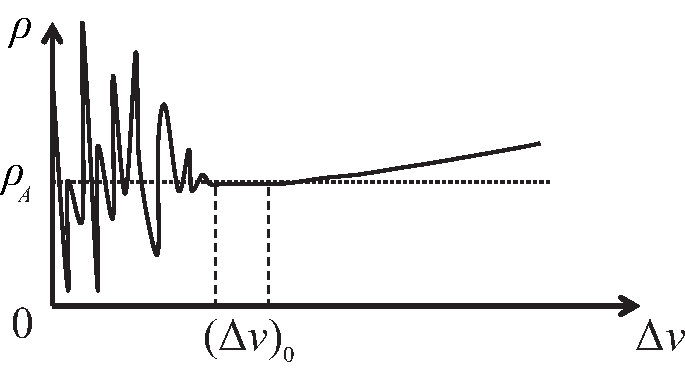
\includegraphics[width=0.4\linewidth]{pic/连续密度.pdf}
	\vspace*{-0.5em}
	\caption{连续密度示意图}
	\label{连续密度}
\end{figure}

连续介质假设的提出,可以把流体一切宏观物理性质(密度、压强、温度、速度等)表达为空间和时间的连续可微函数,便于用数学分析工具来解决问题。

\subsection{流体的易流动性}
\vspace*{-1em}

\begin{figure}[!htb]
	\begin{minipage}{0.5 \linewidth}
		\centering
		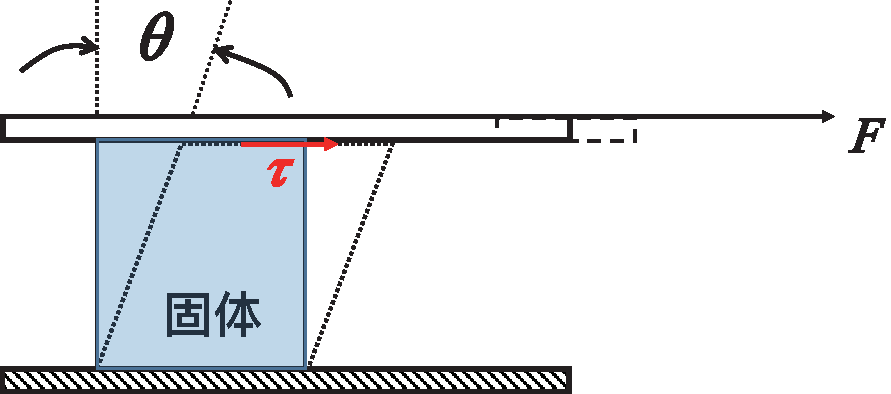
\includegraphics[width=0.8\linewidth]{pic/固体流动.pdf}
		\caption{固体所受剪力}
		\label{固体流动}
	\end{minipage}
	\begin{minipage}{0.5 \linewidth}
		\centering
		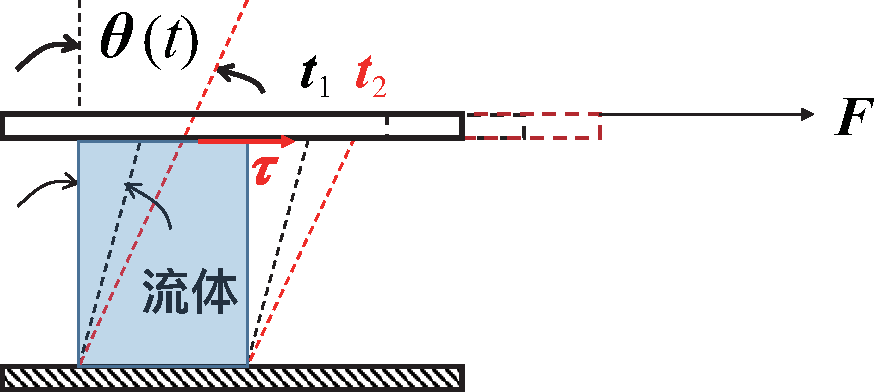
\includegraphics[width=0.8\linewidth]{pic/流体流动.pdf}
		\caption{流体所受剪力}
		\label{流体流动}
	\end{minipage}
\end{figure}
\vspace*{-1em}

\begin{itemize}
	\item 如图\ref{固体流动}所示,固体能够靠产生一定的剪切角变形量$\theta$来抵抗剪切应力$\tau$.\vspace*{-1em}
	
	\item 如图\ref{流体流动}所示,对流体(例如甘油)作类似实验将发现流体的角变形量不仅与剪切应力$\tau$大小有关 而且与剪切应力$\tau$的持续时间$t$长短有关 。
\end{itemize}
\vspace*{-1em}

\defination[流体的易流动性]
{
	流体的\dy[易流动性]{YLDX}是指不论所加剪切应力$\tau$多么小,只要不等于零,流体都将在剪应力作用下持续不断的产生变形运动流动的特性。
}

流体是\red[连续且具有易流性的物质],在静止状态下不能承受剪应力,而固体在静止状态下可以承受一定强度的剪切应力。这是流体和固体在宏观受力的本质区别。

\subsection{流体的压缩性和弹性}
\vspace*{-1em}
\defination[流体的压缩性和弹性]
{流体受压时其体积发生改变的性质成为流体的\dy[压缩性]{YSX},而抵抗压缩变形的能力或特性称为\dy[弹性]{TX}。}

\defination[压缩性系数]
{\dy[压缩性系数]{YSXXS}定义为单位压强差所产生的相对体积改变量
\begin{equation}
	\beta_p = - \dfrac{\d v / v}{\d p},\quad \left(\dfrac{1}{\text{N}/\text{m}^2}\right)
\end{equation}
}
压缩性系数反映的是流体受压的简单程度。

\defination[体积弹性模量]
{\dy[体积弹性模量]{TJTXML}定义为产生单位相对体积改变量所需的压强增量
\begin{equation}
	E = \dfrac{\d p}{\d v / v} =  \dfrac{1}{\beta_p}, \qquad \left(\text{N} / \text{m}^2\right)
\end{equation}
}
体积弹性模量反映的是流体受压的难度。

液体的体积弹性模量一般较大,通常可视为不可压缩流体。而气体的体积弹性模量一般较大且与热力学过程有关,所以通常视为可压缩流体。

\defination[马赫数]
{\dy[马赫数]{MHS}定义为飞行器的飞行速度$u$和声速$a$的比值
\begin{equation}
	M_a = \frac{u}{a}
\end{equation}}

马赫数的大小可以看成是\blue[气体相对压缩性]的一个指标。在考虑具体流动时,一般按照速度(马赫数)大小将流动划分为不可压缩流动和可压缩流动。当$M_a < 0.3$时,气体流动的可压缩性影响可以忽略不计。
\vspace*{0.5em}

\subsection{流体的粘性}
由于流体粘性影响,均匀流经平板时,贴着平板表面的流体速度降为零,称为\red{流体与板面间 “无滑移” 边界条件}。由于收到内层流体的摩擦力、外层流体的速度有变慢趋势,反过来,由于收到外层流体的摩擦力,内层流体的速度有变快趋势。流层简单“互相牵扯”作用一层层向外传递,在距离板面一定距离后,这种作用逐步消失,速度分布变为均匀。

\defination[流体粘性]
{流层之间“阻碍”流体相对变形趋势的能力称为\dy[流体粘性]{LTNX},相对错动(剪切)流层间的一对摩擦力即\dy[粘性剪切力]{NXJQL}。}

\begin{figure}[!htb]
	\centering
	\begin{minipage}{0.45 \linewidth}
		\centering
		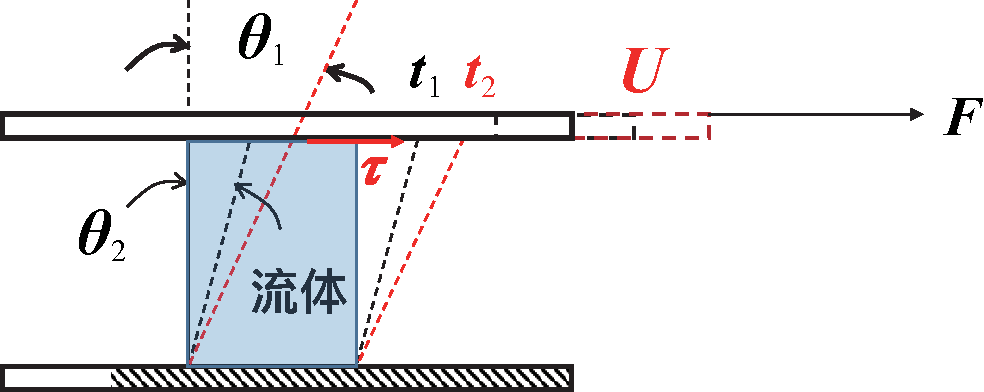
\includegraphics[width=\linewidth]{pic/流体粘性实验.pdf}
		\caption{流体剪切实验}
		\label{流体剪切实验}
	\end{minipage}
	\begin{minipage}{0.45 \linewidth}
		\centering
		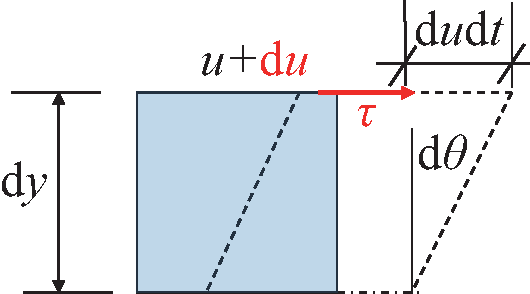
\includegraphics[width=0.7\linewidth]{pic/粘性几何关系.pdf}
		\vspace*{0.1em}
		\caption{流体剪切几何关系}
		\label{流体剪切几何关系}
	\end{minipage}
\end{figure}
\vspace*{-1em}

如图\ref{流体剪切实验}所示,可以得到剪切力和粘性剪切应力的表达式
\begin{equation}
	F = \mu \dfrac{U}{h}A, \qquad \tau = \dfrac{F}{A} = \mu \dfrac{U}{h}
\end{equation}

\theorem[牛顿粘性应力公式]
{
	\quad \vspace*{-1em}
	\begin{equation}
		\tau = \mu \dfrac{\d u}{\d y}
		\label{牛顿粘性应力公式}
	\end{equation}
	其中,$\mu$是流体的粘性系数,$u$是流体的运动速度。\dy[牛顿粘性应力公式]{NDNXYLGS}表明粘性剪切应力不仅与速度梯度有关,而且与物性有关。
}
\noindent 从牛顿粘性应力公式可以看出:\vspace*{-0.5em}
\begin{itemize}
	\item 流体的剪应力与压强$p$无关。\vspace*{-0.5em}
	\item 当$\tau \neq 0$时,$\dfrac{\d u}{\d y} \neq 0$,即无论剪应力多小,只要存在剪应力,流体就会发生变形运动,呈现速度梯度。\vspace*{-0.5em}
	\item $\dfrac{\d u}{\d y}=0$时,$\tau = 0$,即只要流体静止或无变形,就不存在剪应力,流体不存在静摩擦力。
\end{itemize}
因此,\textbf{牛顿粘性应力公式可看成流体易流性的数学表达}。

如图\ref{流体剪切几何关系}所示,可以找到几何关系
\begin{equation}
	\d \theta \d y = \d u \d t , \quad \dfrac{\d \theta }{\d t} = \dfrac{\d u}{\d y}
\end{equation}
即微团垂直线在单位时间内顺时针的转角$=$速度梯度,速度梯度也表示流体微团的\dy[剪切变形速度]{JQBXSD}或\dy[角变形率]{JBXL}。

一般地,流体剪切应力与速度梯度的关系表示为:
\begin{equation}
	\tau = A + B \left(\dfrac{\d u}{\d y}\right)^n
\end{equation}
 但是我们一般只研究\dy[牛顿流体]{NDLT}(如水、空气、汽油、酒精等),即满足牛顿粘性应力公式\eqref{牛顿粘性应力公式}的流体。
 
 \warn[\textbf{液体和气体产生粘性的物理原因不同}\\
\hspace*{2em}液体的粘性主要来自于液体分子间的{\blue[内聚力]},气体的粘性主要来自于气体分子的{\blue[热运动]}。因此液体与气体{\red[动力粘性系数随温度变化的趋势相反]}(气体粘性系数随温度的升高而升高,液体粘性系数随温度的升高而降低),但动力粘性系数与压强基本无关。]
 
\defination[动力学粘性系数和运动学粘性系数]
{
	在许多空气动力学问题里,粘性力和惯性力同时存在,在式子中$\mu$和$\rho$往往以$\dfrac{\mu}{\rho}$的组合形式出现,用符号$\nu$表示:(注意$\mu$和$\nu$的物理区别)
	{
		\begin{itemize}
			\item \dy[动力学粘性系数]{DLXNXXS}:$\mu \quad \left[\dfrac{\text{N}\cdot \text{s}}{\text{m}^2}\right]\qquad \mu_{\text{a}} = 1.7894\times 10^{-5} \, \text{kg/m/s}, \quad \mu_{\text{w}} = 1.139 \times 10^{-3}\, \text{kg/m/s}$  
			
			\item \dy[运动学粘性系数]{YDXNXXS}:$\nu = \dfrac{\mu}{\rho} \quad \left[\dfrac{\text{m}^2}{\text{s}}\right]\qquad \nu_\text{a} = 1.461\times 10^{-5} \, \text{m}^2/\text{s} \quad \nu_\text{w} = 1.139\times 10^{-6} \, \text{m}^2/\text{s}$
		\end{itemize}
	}
}
可以看出:空气动力粘性不大,初步近似研究时可忽略其粘性作用,忽略粘性的流体称为\dy[理想流体]{LXLT}。

\section{作用在流体微团上的力的分类}
\subsection{质量力}
\vspace*{-1.5em}
\defination[质量力]
{
	\dy[质量力]{ZLL}:外力场作用于流体\blue[微团质量中心],\blue[大小与微团质量成正比]的\blue[非接触力]。例如重力,惯性力和磁流体具有的电磁力等都属于质量力 。
}

由于质量力按质量分布,故一般用单位质量的质量力(单位质量力)表示,并写为分量形式:
\begin{equation}
	\bm{f}_v = \lim \dfrac{\Delta \bm{F}_v}{\rho \Delta v} = f_x \bm{i} + f_y \bm{j} + f_z \bm{k}
\end{equation}
其中,$\Delta v$是微团体积,$\rho$是密度,$\Delta \bm{F}_v$为作用于微团的质量力,$\bm{i}, \bm{j}, \bm{k}$分别是三个坐标方向的单位向量,$f_x, f_y, f_z$分别是三个方向的单位质量力分量。

\begin{figure}[!htb]
	\centering
	\begin{minipage}{0.45 \linewidth}
		\centering
		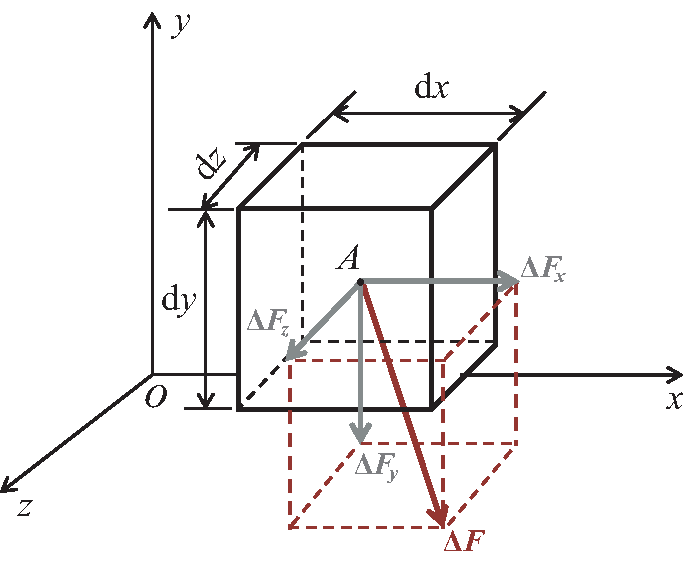
\includegraphics[width=\linewidth]{pic/质量力.pdf}
		\caption{质量力的分解}
		\label{质量力}
	\end{minipage}
	\begin{minipage}{0.45 \linewidth}
		\centering
		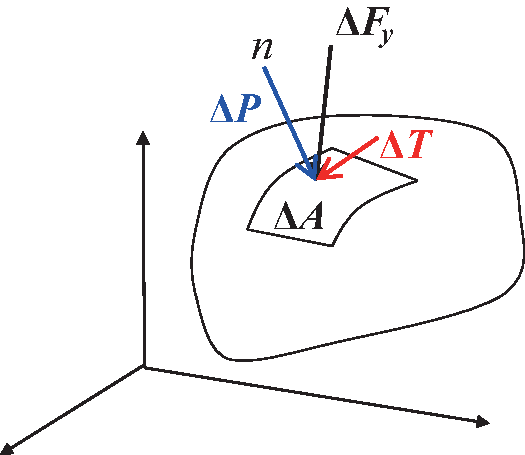
\includegraphics[width=0.8\linewidth]{pic/表面力.pdf}
		\vspace*{2.6em}
		\caption{表面力的分解}
		\label{表面力}
	\end{minipage}
\end{figure}

\subsection{表面力}
\vspace*{-1em}

\defination[表面力]
{
	\dy[表面力]{BML}:相邻流体或物体作用于所研究流体团块外表面,大小与流体团块表面积成正比的接触力。由于按面积分布,故用接触应力表示,并可将其分解为法向应力和切向应力。\vspace*{-0.5em}
	{
		\begin{itemize}
			\item 法向应力(正应力)
			\begin{equation}
				p = \lim\limits_{\Delta A \to 0} \dfrac{\Delta P}{\Delta A}
			\end{equation}
			
			\item 切向应力(切应力)
			\begin{equation}
				\tau = \lim\limits_{\Delta A \to 0} \dfrac{\Delta T}{\Delta A}
			\end{equation} 
		\end{itemize}
	}
}

\noindent 流体内任取一个剖面一般有法向应力和切向应力,但切向应力完全是由粘性产生的 。\vspace*{-0.5em}

\begin{itemize}
	\item \blue[静止流体]:内部任意一点的应力只有内法向应力。\vspace*{-0.5em}
	\item \blue[无粘理想流体]:内部任意一点只有法向应力,而没有切向应力 。\vspace*{-0.5em}
	\item \blue[粘性流体]\vspace*{-0.5em}
	\begin{itemize}
		\item 在静止状态下:其内部任意一点的应力只有内法向应力;\vspace*{-0.5em}
		\item 在运动状态下:其内部任意一点的应力除法向应力外,还有切向应力。
	\end{itemize}
\end{itemize}


\section{静止流体内任一点压强的各向同性特征}
\subsection{压强的定义}
\vspace*{-1em}

\defination[压强]
{
	理想(无粘)流体中的法向应力称为\dy[压强]{YQ},其指向沿
表面的内法线方向,压强的量纲是$[\mbox{力}]/[\mbox{长度}]^2$,单位为$(N/m^2)$或帕Pa.
	\begin{equation}
		p = \lim\limits_{\Delta A \to 0} \dfrac{\Delta P}{\Delta A}
	\end{equation}
}




\subsection{压强的各向同性}

\begin{figure}[!htb]
	\centering
	\begin{minipage}{0.4 \linewidth}
		\centering
		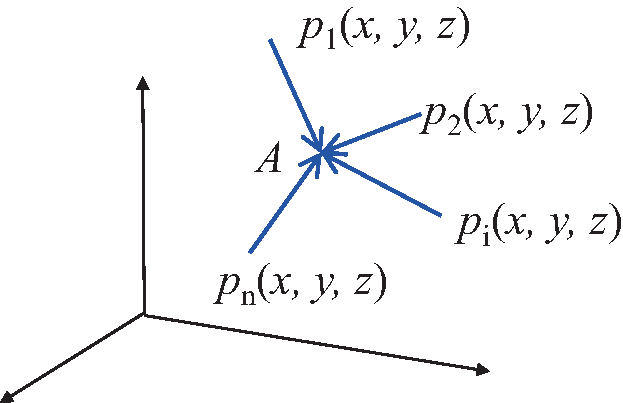
\includegraphics[width=0.9\linewidth]{pic/压强各向同性1.pdf}
		\caption{压强各向同性示意图}
		\label{压强各向同性}
	\end{minipage}
	\begin{minipage}{0.5 \linewidth}
		\centering
		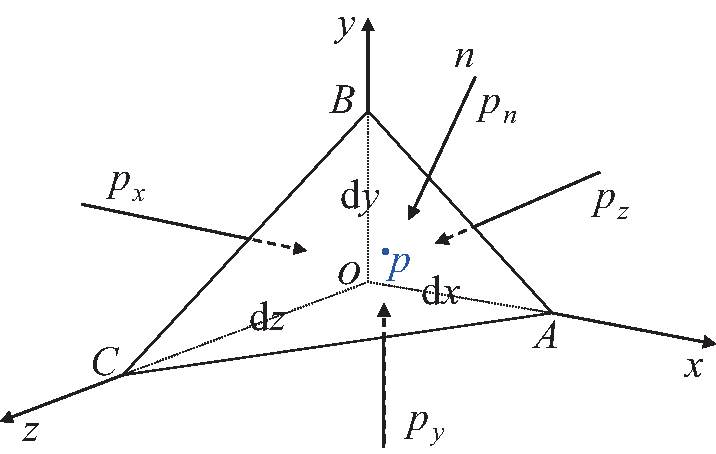
\includegraphics[width=0.8\linewidth]{pic/压强各向同性2.pdf}
		\vspace*{-1em}
		\caption{微元四面体压强分析}
		\label{压强各向同性证明}
	\end{minipage}
\end{figure}

如图\ref{压强各向同性证明},考虑微元四面体$ABCO$中心压强$p$,对于$x$方向,有
\begin{equation*}
	p_x \dfrac{1}{2} \d y \d z - p_n \d s \cos(\bm{n}, \bm{x}) = \rho \dfrac{1}{6} \d x \d y \d z a_x
\end{equation*}
由于$\d x \d y \d z $是高阶无穷小量,忽略后得
\begin{equation*}
	p_x \dfrac{1}{2} \d y \d z - p_n \d s \cos(\bm{n}, \bm{x}) = 0 \quad \Longrightarrow \quad p_x = p_n
\end{equation*}
同理,对$y,z$方向也可以得到类似的结果。所以,我们得到压强各个方向都相等的结论。

\theorem[压强各向同性]
{
	如图\ref{压强各向同性}所示,在理想(无粘)流体中,不论流体静止还是运动,尽管一般压强是位置的函数$p = p(x, y, z)$, 但在同一点处压强不因受压面方位不同而变化,这个特性称为\dy[压强各向同性]{YQGXTX},即
	\vspace*{-1em}
	\begin{equation}
		p_1 = p_2 = p_3 = p_x = p_y = p_z =p_i = p_n
	\end{equation}
}

\subsection{压强属性}
\begin{itemize}
	\item \blue[静止流体]:内部任意一点的应力只有内法向应力,即压强。\vspace*{-0.5em}
	\item \blue[无粘理想流体]:内部任意一点只有法向应力,而没有切向应力,即压强。\vspace*{-0.5em}
	\item \blue[粘性流体]\vspace*{-0.5em}
	\begin{itemize}
		\item 在静止状态下:其内部任意一点的应力只有内法向应力,即压强;\vspace*{-0.5em}
		\item 在运动状态下:其内部任意一点的应力除法向应力外,还有切向应力。因此,\red[粘性流体的压强严格说指的是三个互相垂直方向的内法向应力的平均值]。
	\end{itemize}
\end{itemize}

\noindent 压强的单位\footnote{$1 \, \text{Torr}$:$0\degree \text{C}$标准重力下,1 $\,$mmHg柱的压力;$1 \, \text{psi}$:磅每平方英寸。}及其换算如下
\begin{equation}
	\begin{split}
			1 \, \text{ba} &= 10^5 \, \text{Pa} = 10^3 \, \text{mba} \\
			1 \, \text{atm} = 101300 \, \text{Pa}&= 101.3 \, \text{kPa} = 1.013 \, \text{ba} = 1013 \, \text{mba}\\
			1 \, \text{Torr} &= 133.3 \, \text{Pa}\\
			1 \, \text{psi} &= 6896.6 \, \text{Pa}
	\end{split}
\end{equation}

\section{流体静平衡微分方程}
\subsection{压强在静平衡流体中的分布规律}

\begin{figure}[!htb]
	\centering
	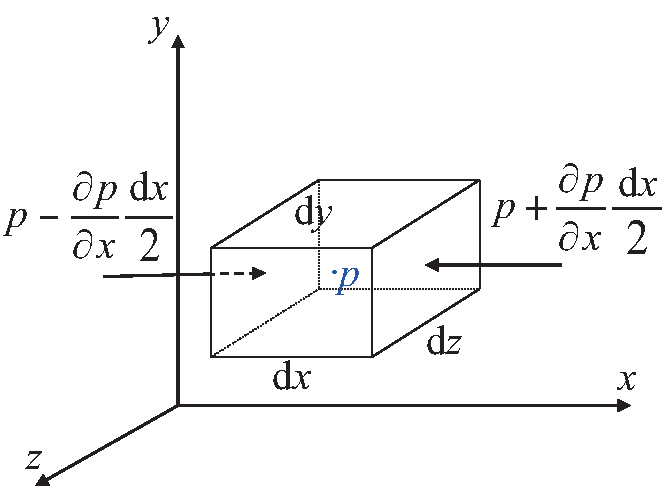
\includegraphics[width=0.35\linewidth]{pic/压强静平衡.pdf}
	\vspace*{-1em}
	\caption{微元六面体压强分析}
	\label{压强静平衡方程推导}
\end{figure}

以平衡流体内的任意一个六面体微元$\d V = \d x \d y \d z$为分析对象,中心点的压强为$p = p(x,y,z)$,密度为$\rho = \rho (x,y,z)$,三个方向的单位质量的质量力$f_x, f_y, f_z$。

由于流体静止、六面体微元表面无剪应力,只受到法相应力(即压力),用中心点处压强$p$的一阶泰勒展开表示,即
\begin{equation}
	P(x) = \dfrac{p}{0!} + \dfrac{P'(x)}{1!}(x - x_0) + \dfrac{P''(x_0)}{2!}(x - x_0)^2 + \cdots + \dfrac{P^{(n)}(x_0)}{n!}(x-x_0)^n + R_n(x) \approx p + \dfrac{\partial p}{\partial x} (x - x_0)
\end{equation}

\begin{itemize}
	\item $x$方向的表面力为:$\left(p - \dfrac{\partial p}{\partial x}\cdot \dfrac{\d x}{2}\right)\d y \d z  - \left(p + \dfrac{\partial p}{\partial x}\cdot \dfrac{\d x}{2}\right)\d y \d z= - \dfrac{\partial p}{\partial x}\d x \d y \d z$
	\item $x$方向的质量力为:$f_x\rho \d x \d y \d z$
	\item 由静平衡态合力为0,得
	\begin{equation}
		- \dfrac{\partial p}{\partial x}\d x \d y \d z + f_x\rho \d x \d y \d z = 0 \quad \Rightarrow \quad \dfrac{\partial p}{\partial x} = \rho f_x
	\end{equation}
\end{itemize}
同理可得到$y,z$方向上的静平衡方程,综合可得

\theorem[欧拉平衡微分方程组]
{
	\quad \vspace*{-1em}
	\begin{equation}
		\begin{cases}
			\, \dfrac{\partial p}{\partial x} = \rho f_x\\[0.5em]
			\, \dfrac{\partial p}{\partial y} = \rho f_y\\[0.5em]
			\, \dfrac{\partial p}{\partial z} = \rho f_z
		\end{cases}
		\quad \Longleftrightarrow \quad \nabla p = \rho \bm{f}
		\label{PH}
	\end{equation}
	其中,$\nabla = \dfrac{\partial }{\partial x}\bm{i} + \dfrac{\partial }{\partial y}\bm{j} + \dfrac{\partial }{\partial z}\bm{k}$为矢量微分算子,也称\dy[哈密顿算子]{HMDSZ}。
}
其物理意义为:当流体平衡时,若压强在某个方向存在梯度的话,必然是由质量力在该方向有分量造成的。而且,沿质量力方向压强增加。

将\eqref{PH}分别乘以$\d x, \d y, \d z$并相加得到
\begin{equation}
	\begin{cases}
		\, \dfrac{\partial p}{\partial x}\,\d x = \rho f_x \, \d x\\[0.5em]
		\, \dfrac{\partial p}{\partial y} \, \d y= \rho f_y \, \d y\\[0.5em]
		\, \dfrac{\partial p}{\partial z}\, \d z = \rho f_z \, \d z
	\end{cases}
	\quad \Longrightarrow \quad 
	\dfrac{\partial p}{\partial x}\,\d x + \dfrac{\partial p}{\partial y} \, \d y + \dfrac{\partial p}{\partial z}\, \d z = \rho \big(f_x \, \d x + f_y \, \d y + f_z \, \d z\big)
	\label{PH1}
\end{equation}
式子\eqref{PH1}左边为全微分$\d p = \dfrac{\partial p}{\partial x}\,\d x + \dfrac{\partial p}{\partial y} \, \d y + \dfrac{\partial p}{\partial z}\, \d z$,即
\begin{equation}
	\d p = \rho \big(f_x \, \d x + f_y \, \d y + f_z \, \d z\big)
\end{equation}
式子\eqref{PH1}右边若满足(充要条件)
\begin{equation}
	\dfrac{\partial f_x}{\partial y} = \dfrac{\partial f_y}{\partial x} \quad \dfrac{\partial f_y}{\partial z} = \dfrac{\partial f_z}{\partial y} \quad \dfrac{\partial f_z}{\partial x} = \dfrac{\partial f_x}{\partial z} 
\end{equation}
那么式子\eqref{PH1}右边也是某个函数的全微分,这个函数记为$\Omega = \Omega(x,y,z)$,称为\dy[质量力的势函数]{ZZLDSHS},并设
\begin{equation*}
	f_x = - \dfrac{\partial \Omega}{\partial x}, \qquad f_y = - \dfrac{\partial \Omega}{\partial y}, \qquad f_z = - \dfrac{\partial \Omega}{\partial z} \quad \Longleftrightarrow \quad \bm{f} = - \nabla \Omega
\end{equation*}
则静平衡方程也可以写为
\begin{equation}
	\d p = - \rho \d \Omega
	\label{压强静平衡方程}
\end{equation}
沿空间任意闭曲线$C$进行积分:
\begin{equation}
	\text{LHS} \quad \oint_{C} \d p = 0 \qquad \Longrightarrow \qquad \text{RHS} \quad \oint_{C} - \rho \, \d \Omega = 0
\end{equation}

这说明\textbf{作用在流体质点上的质量力积分与路径无关}。即\blue[质量力是有势力]。由此得到,在静止状态下,流体所受的质量力必须是有势力 。 

当密度$\rho$为常数(如不可压流体)时,对流体静平衡微分方程\eqref{压强静平衡方程}进行积分,得
\begin{equation}
	p = - \rho \Omega + C
\end{equation}
如果知道流体中某一点$a$的压强值$p_a$ 和质量力势函数$\Omega_a$的值,则任何其它点的压强和势函数的关系为
\begin{equation}
	p = p_a - \rho \left(\Omega - \Omega_a\right)
\end{equation}

\subsection{等压面}
\vspace*{-1em}
\defination[等压面]
{
	\dy[等压面]{DYM}:流场中压强相等的空间点组成的几何曲面或平面。
}

由等压面的定义,可以得到

\theorem[等压面微分方程]
{
	\quad \vspace*{-1em}
	\begin{equation}
		\begin{cases}
			\, p = \text{constant}\\
			\, \d p = 0\\
			\, f_x  \d x + f_y \d y + f_z \d z = 0 \qquad (\d \Omega = 0)
		\end{cases}
	\label{等压面微分方程}
	\end{equation}
	对\eqref{等压面微分方程}进行积分可以得到一个满足$\d p = 0$对几何曲面,所以公式\eqref{等压面微分方程}称为\dy[等压面微分方程]{DYMWFFC}。
}
\vspace*{-0.5em}

等压面上质量力不作功($\d \Omega = 0$),质量力在等压面上的投影为0(等压面满足$f_x  \d x + f_y \d y + f_z \d z = 0$)。
\section{标准大气}

 \subsection{地球大气的分层}
\begin{equation*}
	\mbox{地球大气层}\,
	\begin{cases}
		\, \mbox{高层大气}\,
			\begin{cases}
				\, \mbox{外层大气} \qquad  > 400  \, \text{km}\\[0.5em]
				\, \mbox{高温层} \qquad  80 \, \text{km} \, \sim 400 \, \text{km} \\
			\end{cases}\\[2em]
	\, \mbox{低层大气}\,
			\begin{cases}
				\, \mbox{中间大气层} \qquad 32 \, \text{km} \, \sim 80 \, \text{km}\\[0.5em]
				\, \mbox{平流层(同温层)}\quad \, \text{对流层顶部} \, \sim 32 \, \text{km}\\[0.5em]
				\, \mbox{对流层}
					\begin{cases}
						\, \mbox{赤道处}\qquad 0 \, \sim \, (16 - 18)\, \text{km}\\
						\, \mbox{中高纬度} \qquad 0 \, \sim \, (8 - 12)\, \text{km}
					\end{cases}
			\end{cases}
	\end{cases}
\end{equation*}

\begin{enumerate}
	\item \dy[对流层]{DLC}(Troposphere) \vspace*{-0.5em}
	\begin{itemize}
		\item 高度$ 8\, \sim \,  18 \,\text{km} $随纬度变化 
		\item 密度大 占总质量的$\dfrac{3}{4}$ 
		\item 空气有上下流动,存在气象活动(雷雨风暴) 
		\item 温度随高度增加而线性降低
		\item 与平流层之间存在\dy[对流层顶]{DLCD}(Tropopause)
	\end{itemize}
	
	\item \dy[平流层]{PLC}(Stratosphere) \vspace*{-0.5em}
	\begin{itemize}
		\item 高度$ 12\, \sim \,  32 \,\text{km} $
		\item 占总质量的$\dfrac{1}{4}$
		\item 大气仅做水平运动 
		\item 从对流层顶部至$ 20 \, \text{km}$,温度为常数;$20 \, \text{km} \, \sim 32 \, \text{km}$ ,温度随高度有所上升
		\item 顶部压强约为海平面值的千分之一
	\end{itemize}
	
	\item \dy[中间大气层]{ZJDQC}(Mesosphere) \vspace*{-0.5em}
	\begin{itemize}
		\item 高度$ 32\, \sim \,  80 \,\text{km} $
		\item 占总质量的$\dfrac{1}{3000}$ 
		\item 温度随高度增加先升后降
		\item \dy[临近空间]{LJKJ} 
			\begin{itemize}
				\item $20 \, \text{km} \, \sim \, 100 \, \text{km}$,包括平流层绝大部分区域 、中间层的全部和高温层的底部。
				\item 低雷诺数问题
			\end{itemize}
	\end{itemize}
	
	\item \dy[高温层]{GWC}(Thermosphere) \vspace*{-0.5em}
	\begin{itemize}
		\item 高度$ 80\, \sim \,  400 \text{km} $
		\item 由于太阳短波辐射的缘故,温度随高度而上升
		\item 空气分子发生电离
		\item $100 \, \text{km}$以上高空的空气为良导体
		\item 高度$> 150 \, \text{km}$,空气过于稀薄,声波无法产生与传播
	\end{itemize}
	
	\item \dy[外层大气]{GWC}(Exosphere) \vspace*{-0.5em}
	\begin{itemize}
		\item 高度$ >  400 \text{km} $
		\item 空气十分稀薄,没有常规温度定义
		\item 空气分子可逸入太空而不与其他分子发生碰撞
		\item 分子平均自由程$l$可以达到数百公里
		\item 占大气总质量的$10^{-11}$
		\item 包含大部分卫星运行轨道
	\end{itemize}
	
\end{enumerate}

\subsection{温度变化曲线}

\begin{itemize}
	\item 对流层$ 0\, \sim \,  11 \,\text{km} $
	\begin{equation}
		T = 288.15 - 0.0065H
	\end{equation}
	6
	\item 平流层$ 11\, \sim \,  32 \,\text{km} $
	\begin{itemize}
		\item $H = 11 \, \sim \, 20 \, \text{km}$
		\begin{equation}
			T = 216.65
		\end{equation}
		\item $H = 20 \, \sim \, 32 \, \text{km}$
		\begin{equation}
			T = 216.65 + 0.001(H - 20000)
		\end{equation}
	\end{itemize}
\end{itemize}

{
	\centering
\begin{minipage}{0.7\linewidth}
	\subsection{静态压强变化}
	\hspace*{2em} 如图\ref{空气柱}所示,去厚度为$\d y$的空气柱片进行分析
	\begin{equation}
		\dfrac{\d p}{\d y} = - g \rho \qquad \xrightarrow{\quad \textstyle \rho = \dfrac{p}{RT} \quad } \qquad \dfrac{\d p}{\d y} = - \dfrac{g \rho }{RT}
	\end{equation}
	其中,如果已知$g,T$随着高度$y$的变化关系,就可以积分得到压强$p$随着高度$y$的变化关系。
	
	\hspace*{2em}$g$随高度的变化规律为
	\begin{equation*}
		\dfrac{g}{g_0} = \left(\dfrac{r}{r+y_g}\right)^2, \qquad r \approx 6400\, \text{km}
	\end{equation*}
\end{minipage}
\begin{minipage}{0.3\linewidth}
		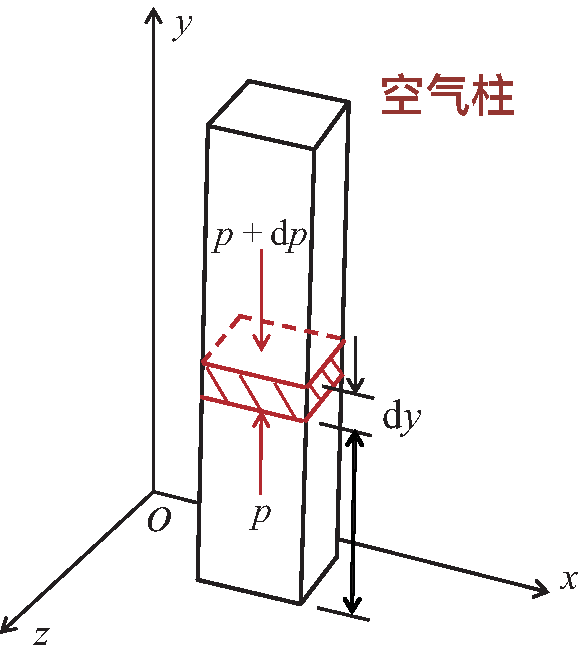
\includegraphics[width=\linewidth]{pic/空气柱.pdf}
		\captionof{figure}{空气柱薄片}
		\label{空气柱}
\end{minipage}
}

\noindent 由此可知,$g$在近地面处可视为常数。

\begin{itemize}
	\item 对流层$ 0\, \sim \,  11 \,\text{km} $
	\begin{equation*}
		\begin{cases}
			\, T = 288.15 - 0.0065y\\
			\, \dfrac{\d p}{\d y} = - \dfrac{gp}{RT}
		\end{cases}
		\quad \Rightarrow \quad \dfrac{\d p}{p} = -\dfrac{g}{R}\dfrac{\d y}{288.15 - 0.0065y}
	\end{equation*}
	即
	\begin{equation}
		\dfrac{p}{p_0} = \left(\dfrac{288.15 - 0.0065y}{288.15}\right) = \left(\dfrac{T}{T_0}\right)^{5.25588},\qquad \dfrac{\rho}{\rho_0} = \dfrac{p}{p_0}\dfrac{T_0}{T} = \left(\dfrac{T}{T_0}\right)^{4.25588}
	\end{equation}
	\item 平流层$ 11\, \sim \,  32 \,\text{km} $
	\begin{itemize}
		\item $H = 11 \, \sim \, 20 \, \text{km}$
		\begin{equation}
			\begin{cases}
				\, T = 216.65\\
				\, \dfrac{\d p}{\d y} = - \dfrac{gp}{RT}
			\end{cases}
		\quad \Rightarrow \quad 
		\dfrac{p}{p_{11}} = \dfrac{\rho}{\rho_{11}}=\e^{\textstyle \frac{y-11000}{6341.62}}
		\end{equation}
		\item $H = 20 \, \sim \, 32 \, \text{km}$
		\begin{equation}
			\dfrac{p}{p_{20}} = \left(\dfrac{T}{216.65}\right)^{-34.1632} \qquad \dfrac{\rho}{\rho_{20}} = \left(\dfrac{T}{216.65}\right)^{-35.1632}
		\end{equation}
	\end{itemize}
\end{itemize}



